\documentclass[a4paper,12pt]{article}
 
% packages
\usepackage[T1]{fontenc}
\usepackage[latin1]{inputenc}
\usepackage{amsmath}
\usepackage{amsfonts}
\usepackage{amssymb}
\usepackage{graphicx}
\usepackage{listings}
\usepackage{url}
\usepackage{color}
\usepackage[top=3cm, bottom=3cm, left=3cm, right=3cm]{geometry}

% Title page definition

\makeatletter
\def\maketitle{%
  \null
  \thispagestyle{empty}%
  \begin{center}\leavevmode
    \normalfont
    {}
    \vskip 1.3cm
    {\Huge \@title\par}%
    \vskip 0.3cm
    {\Large Version: 0.8.0\par}%
    \vskip 0.3cm
    {\Large \@author\par}%
    \vskip 2cm
    {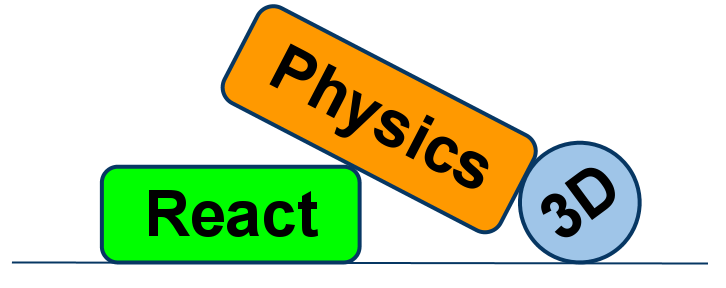
\includegraphics[height=5cm]{images/ReactPhysics3DLogo.png}}
    \vskip 2cm
    {\large{\url{http://www.reactphysics3d.com}}}
    \vskip 0.2cm
   {\large \@date}%
  \end{center}%
  \vfill
  \null
  \cleardoublepage
  }
\makeatother


\begin{document}
   \author{Daniel Chappuis}
   \title{ReactPhysics3D library \\ User Manual}
   \maketitle

   \tableofcontents

   \newpage
 

   \section{Introduction}

  ReactPhysics3D is an open source C++ physics engine library that can be used
  in 3D simulations and games. The library is released under the ZLib license.

   \section{Features}

   The ReactPhysics3D library has the following features :

   \begin{itemize}
    \item Rigid body dynamics 
    \item Discrete collision detection 
    \item Collision shapes (Sphere, Box, Cone, Cylinder) 
    \item Broadphase collision detection (Sweep and Prune using AABBs) 
    \item Narrowphase collision detection (GJK/EPA) 
    \item Collision response and friction (Sequential Impulses Solver)
    \item Multi-platform (Windows, Linux, Mac OS X)
    \item Documentation (User manual and Doxygen API)
    \item Unit tests
   \end{itemize}

  \section{What's new in this version}

  The current version is version 0.3.0 The following things have been
  added or improved in this new version : \\
   
  \begin{itemize}
    \item The Sweep-and-Prune broad-phase collision detection
      algorithm has been rewritten according to the technique
      described by Pierre Terdiman at
      \url{http://www.codercorner.com/SAP.pdf} to be much more efficient
      than the previous naive implementation.
    \item The contact solver has been rewritten to use the Sequential
      Impulses technique from Erin Catto which is mathematically
      equivalent to the Projected Gauss Seidel technique that was used
      before. The Sequential Impulse technique is more
      intuitive.
    \item Implementation of a dedicated collision detection algorithm for spheres
      against spheres instead of using GJK/EPA algorithm.
    \item Make GJK/EPA algorithm more robust for spheres.
    \item Make possible to use a unique instance of a collision shape
      for multiple rigid bodies.
    \item Change the structure of the code for a better separation
      between the collision detection and the dynamics simulation code.
    \item Create the API documentation using Doxygen
    \item Add Unit tests
   \end{itemize}

    \section{License}

    The ReactPhysics3D library is released under the ZLib license. For more information, read the "LICENSE" file.

    \section{Compilation}
    \label{sec:compilation}

    You can use the CMake software to generate the makefiles or the 
    project files for your IDE. CMake can be downloaded at
    \url{http://www.cmake.org} or using you package-management program
    (apt, yum, \dots) on Linux. Then, you will be able to compile the library to create the static library
    file. In order to use ReactPhysics3D in
    your application, you can link your program with this static library.

    \subsection{Linux and Mac OS X}  

    To build the ReactPhysics3D library, create a folder into which
    you want to build the library. Then go into that folder and run
    the \texttt{cmake} command : \\

    \texttt{cmake \textless path\_to\_library\textgreater \ -G "Unix Makefiles" -DCMAKE\_BUILD\_TYPE=Release} \\

    where \texttt{\textless path\_to\_library\textgreater} must be replaced
    by the path to the library which is the path to the
    \texttt{reactphysics3d-0.3.0/} folder. It is the folder that
    contains the \texttt{CMakeLists.txt} file. This will generate the
    makefiles into your build directory you have created before. Notice that the previous command generates the makefiles to
    compile the library in Release mode. If you wan to generate the makefiles to
    compile in Debug mode, you will have to use the following command : \\

    \texttt{cmake \textless path\_to\_library\textgreater \ -G "Unix Makefiles" -DCMAKE\_BUILD\_TYPE=Debug} \\

   If you also want to build the examples at the same time, you can
   use the following command :  \\

   \texttt{cmake \textless path\_to\_library\textgreater \ -G "Unix Makefiles" -DCMAKE\_BUILD\_TYPE=Release \\
     -DCOMPILE\_EXAMPLES=True } \\

  In order to compile the examples, the GLUT or FREEGLUT library needs to be
  installed on your system if you use Mac OS X. \\

  If you want to build the unit tests, you can use the following
  command : \\

  \texttt{cmake \textless path\_to\_library\textgreater \ -G "Unix Makefiles" -DCMAKE\_BUILD\_TYPE=Debug \\
     -DCOMPILE\_TESTS=True } \\

  Now that you have generated the makefiles with the CMake software,
  you can compile the code to build the static library in the
  \texttt{/lib} folder with the following command in your build directory : \\
    
    \texttt{make}  \\

   This will also compile the examples if you have used the above
   option to do it.

    \subsection{Windows}

     On Windows, you can also use the CMake software to generate the
     files that you will be able to use in your favorite IDE to
     compile the library and examples. \\ 

     First, download the CMake
     software for Windows and install it. Then, run the
     \texttt{cmake-gui} program. The program will ask you for the
     source folder which is the \texttt{reactphysics3d-0.3.0/} folder of
     the library. You will also have to select a folder where you want to
     build the library and the examples. Select any empty folder that
     is on your system. Then, you can click on
     \texttt{Configure}. CMake will ask you to choose an IDE that is on
     your system. For instance, you can select Visual Studio. Then you
     can change the compilation options. For instance, if you want to
     generate the files to compile the examples, you have to check the option
     \texttt{COMPILE\_EXAMPLES}. If you want to compile the unit
     tests, you need to check the option \texttt{COMPILE\_TESTS}.
     Note that compiling the examples
     requires the GLUT or FREEGLUT library to be installed on your system. Once
     this is done, you can click on \texttt{Configure} again and
     finally on \texttt{Generate}. \\ 
    
     Now, if you go into the folder you have chosen to build the
     library, you should be able to open the
     Visual Studio Project that CMake has created and compile the
     ReactPhysics3D library and the examples. 

    \section{Using ReactPhysics3D in your application}

    In order to use the library in your own application, first build
    the static library of ReactPhysics3d as described above to get the
    static library file in the \texttt{/lib} folder. Then, in your code, you have to include
    the ReactPhysics3D header file with the line : \\

    \texttt{\#include "reactphysics3d.h"} \\

    Note that the \texttt{reactphysics3d.h} header file can be found in the
    \texttt{/src} folder of the library. Do not forget to add the
    \texttt{/src} folder in your include directories in order that the
    \texttt{reactphysics3d.h} file is accessible in your code. \\

    Don't forget to also link your application with the ReactPhysics3D
    static library.  \\
  
    Then, you should be able to compile your application using the
    ReactPhysics3D library. You should also take a look at the
    examples and the API documentation to get a better idea of how to use the
    ReactPhysics3D library.

    \section{Examples}

    You can find some OpenGL demos in the \texttt{/examples} folder of
    the library. Follow the instructions described in section
    \ref{sec:compilation} to
    compile the examples. Note that the GLUT or FREEGLUT library is required to
    compile and run the examples.

   \section{API Documentation}

   Some documentation about the API of the code has been generated
   using Doxygen. You will be able to find this documentation in the library archive in the folder \texttt{/documentation/API/html/}. You just
   need to open the \texttt{index.html} file with your favorite web browser.

    \section{Bugs}

    If you find some bugs, do not hesitate to report them on the issue tracker of the ReactPhysics3D website at : \\

    \url{http://code.google.com/p/reactphysics3d/issues/list} \\

    Thanks a lot for reporting the bugs that you find. It will help us to correct and improve the library.
   
\end{document}
